\chapter{系统设计与部署分析}

\section{系统总体架构设计}

\begin{figure}[htbp]
    \centering
    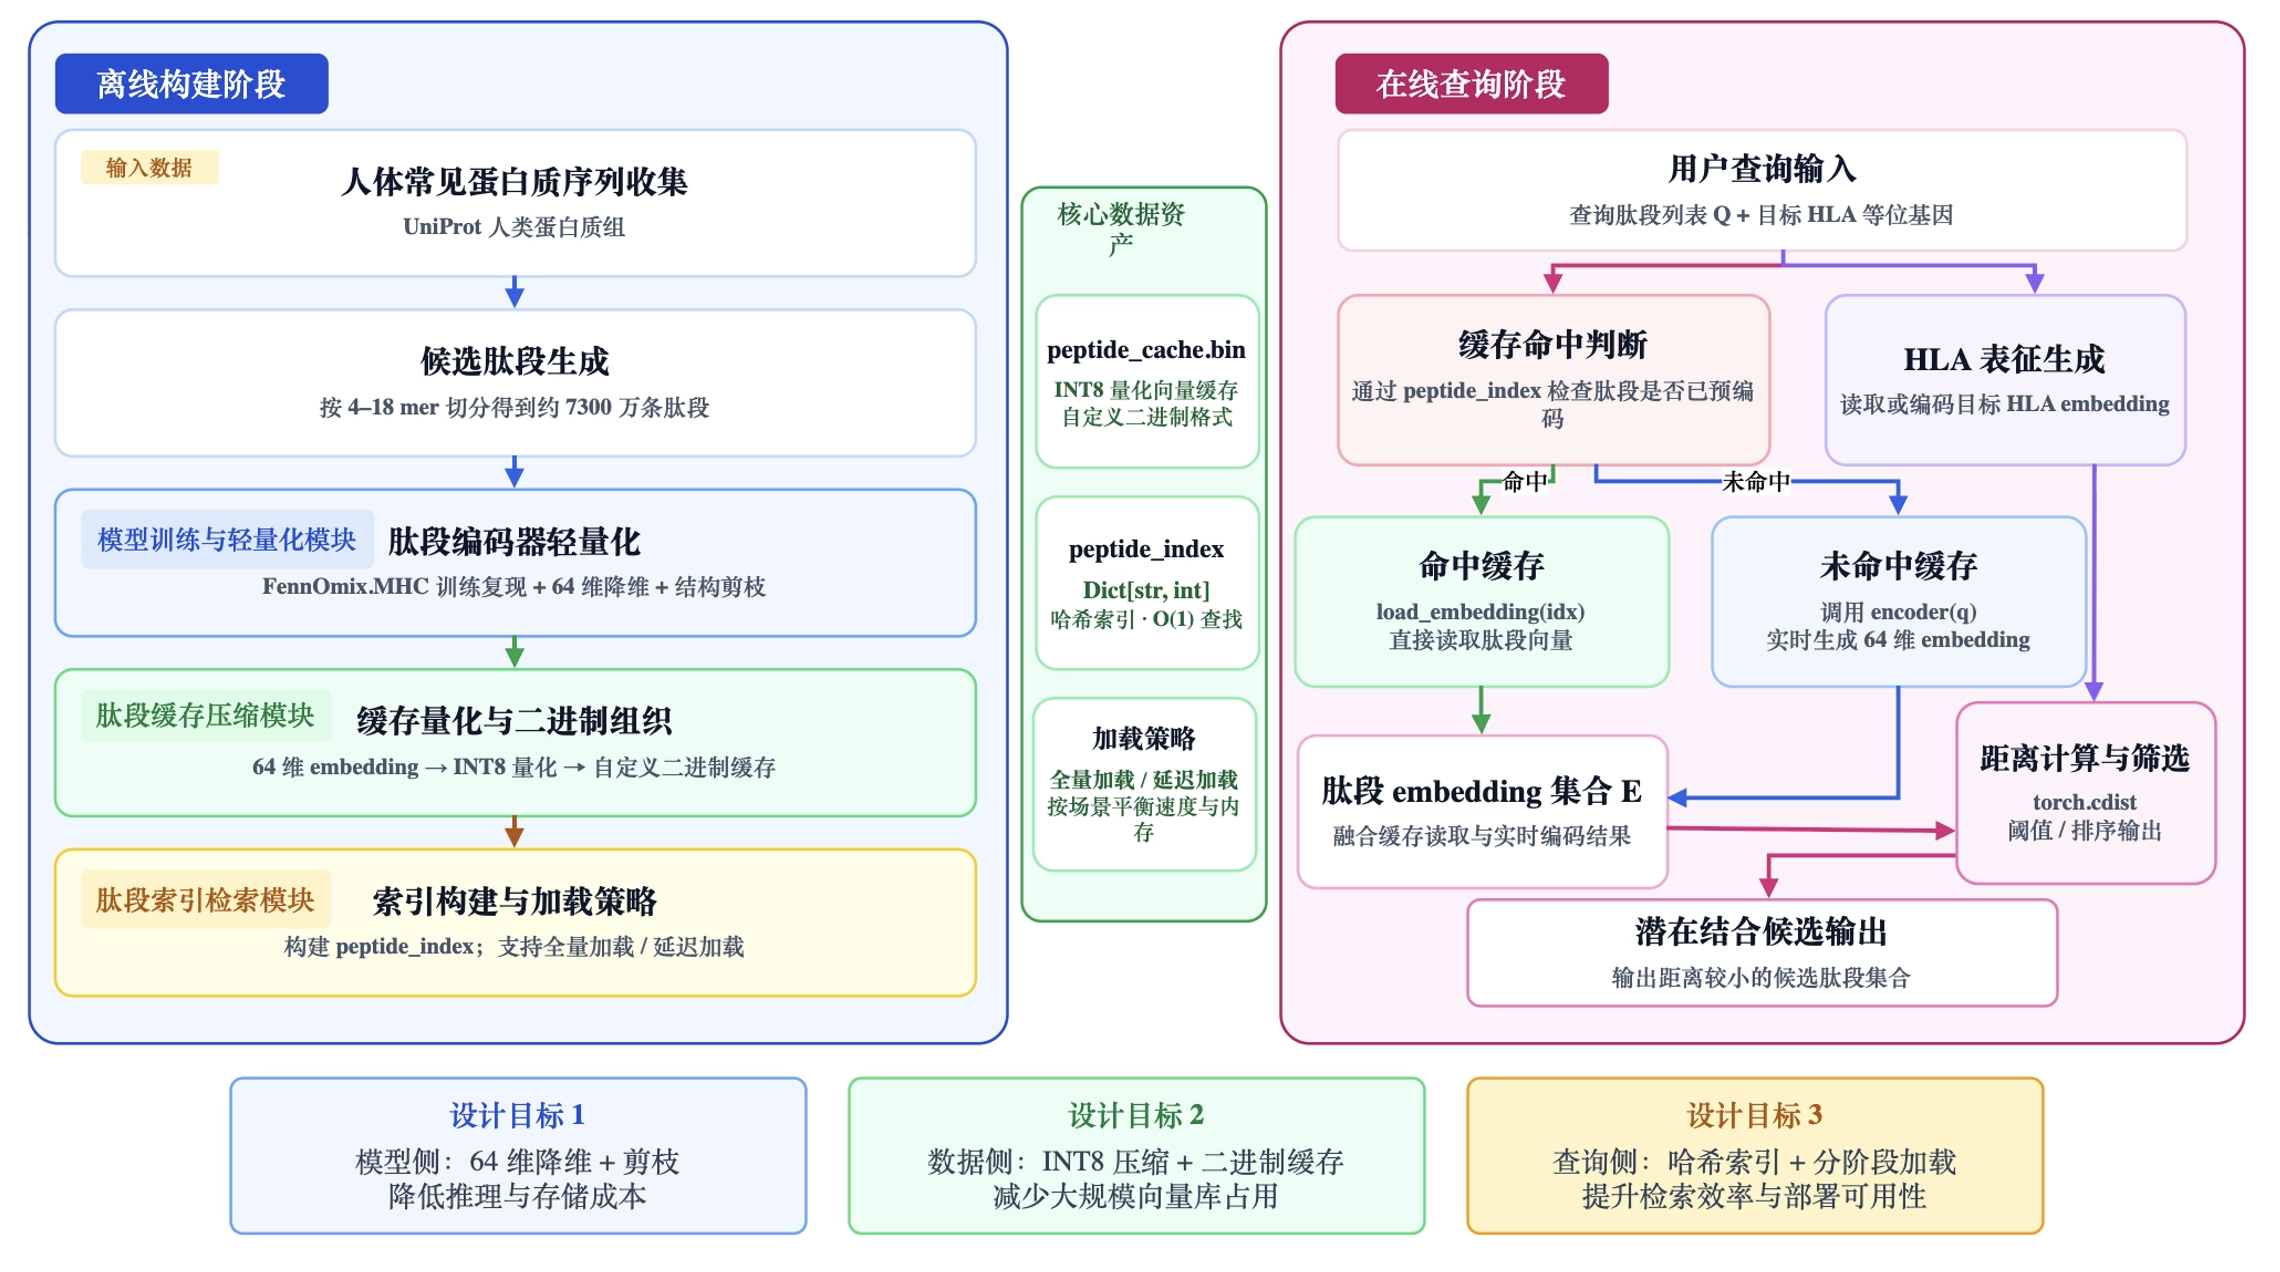
\includegraphics[width=0.95\textwidth]{figures/system_architecture.png}
    \caption{系统总体架构图}
    \label{fig:system-architecture}
\end{figure}

\subsection{系统设计目标}

前文已经从模型轻量化、缓存压缩和索引机制几个方面，验证了在大规模人类蛋白质组场景下优化 FennOmix.MHC 的可行性。本章不再重复具体实验结果，而是聚焦于系统实现与部署，说明这些优化如何被整合成一套可运行的预测和检索流程。

原始模型面对海量候选肽段时，最主要的困难在于在线编码和高维向量检索会带来极高的计算、存储和 I/O 成本。因此，本章系统设计的总体目标是：在保持预测能力的前提下，将模型优化的成果转化为可部署的工程链路，使其能够支撑离线缓存构建、在线快速查询，并在不同资源条件下灵活运行。

这一目标可以拆分为三点：用轻量化模型降低向量生成和推理阶段的计算开销；靠压缩缓存和索引结构压低海量肽段库的存储和访问成本；通过多种加载策略兼顾高频查询和资源受限两类部署场景。于是，本文的系统不再是孤立的模型，而是由模型、缓存、索引和在线查询流程共同组成的一条完整部署链路。

\subsection{离线构建与在线查询流程}

从运行阶段来看，系统可分为离线构建和在线查询两部分。

离线构建阶段负责处理计算量大、但执行频率低的工作。这一步先将候选蛋白序列切割成候选肽段集合，再调用训练好的轻量化肽段编码器生成肽段向量，随后把这些向量写入压缩缓存文件，并同步建立肽段序列到缓存位置的索引映射。目的就是把大批量重复计算前移，为在线查询准备好可复用的数据基础。

在线查询阶段承担实时响应任务。系统拿到输入肽段和目标 HLA 信息后，先通过索引判断该肽段是否已在缓存中：命中则直接读取向量，未命中则调用轻量化编码器实时生成向量。之后，根据肽段向量与 HLA 向量之间的距离关系，给出潜在结合候选。

这种“离线预处理 + 在线快速调用”的划分，有效削减了在线阶段重复推理的开销，使系统在大规模候选库条件下具有更好的响应能力。

\subsection{系统模块划分}

为了便于实现、维护和扩展，系统被拆分为四个核心模块：模型训练与轻量化、肽段缓存压缩、肽段索引检索以及在线预测执行。各模块的功能见表~\ref{tab:system-modules}。

\begin{table}[htbp]
    \centering
    \caption{系统核心模块划分}
    \label{tab:system-modules}
    \begin{tabular}{p{0.24\textwidth} p{0.36\textwidth} p{0.30\textwidth}}
        \toprule
        模块 & 主要功能 & 在系统中的作用 \\
        \midrule
        模型训练与轻量化模块
        & 模型复现、64D 降维、Linear 模型选择与结构剪枝
        & 提供轻量化编码器 \\

        肽段缓存压缩模块
        & 生成并存储压缩后的肽段向量缓存
        & 缓解大规模缓存的存储压力 \\

        肽段索引检索模块
        & 构建肽段到缓存位置的映射，支撑多种加载方式
        & 提升查询定位效率 \\

        在线预测执行模块
        & 执行输入处理、缓存读取、实时编码与距离计算
        & 构成完整的预测服务流程 \\
        \bottomrule
    \end{tabular}
\end{table}

通过这样的划分，模型计算、缓存存储、索引定位和在线预测被解耦成相对独立的功能单元，既降低了耦合度，也为日后单独替换或改进某个模块留下空间。

\section{关键模块实现与协同流程}

\begin{figure}[htbp]
    \centering
    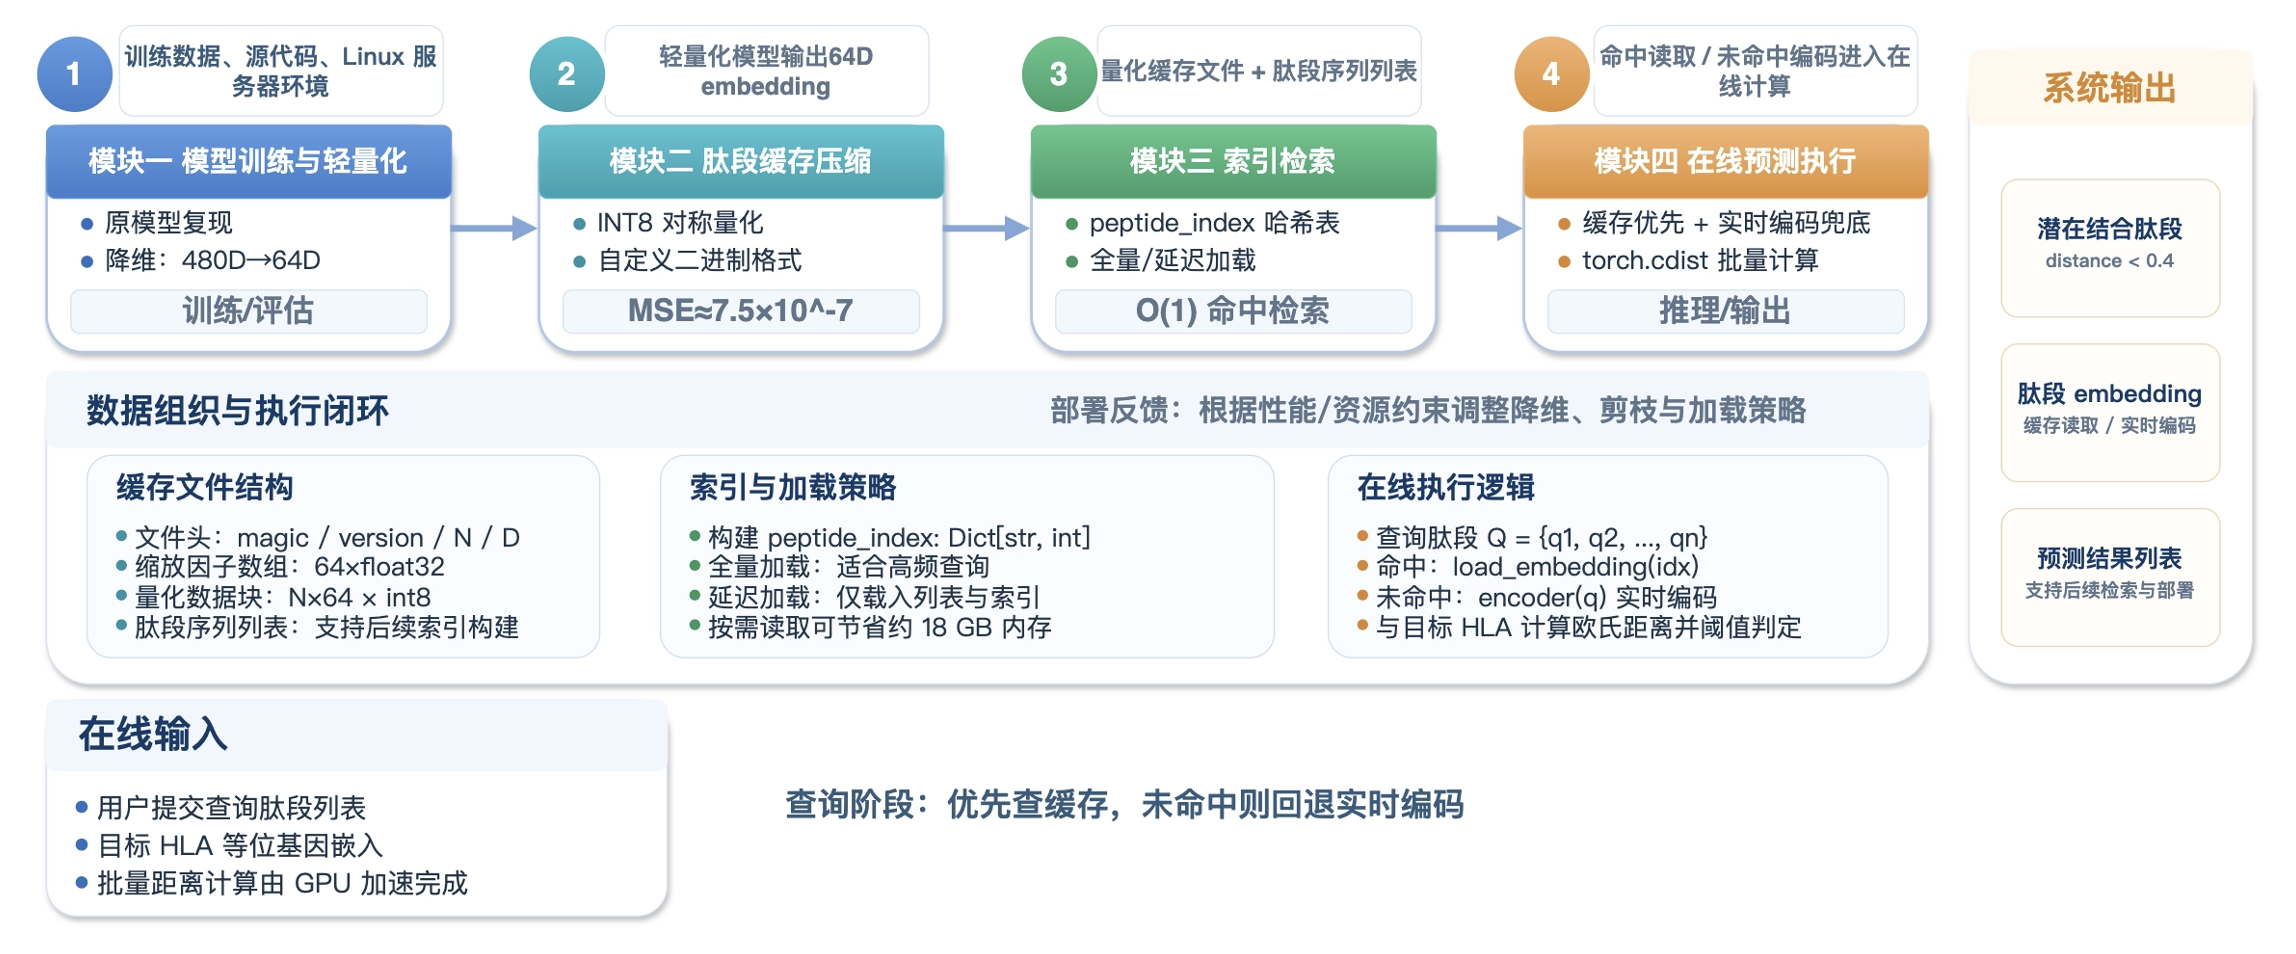
\includegraphics[width=0.95\textwidth]{figures/module_workflow.png}
    \caption{各模块协同流程图}
    \label{fig:module-workflow}
\end{figure}

\subsection{模型训练与轻量化模块}

该模块是整个系统的基础，负责输出可以实际部署的编码器。我们在 FennOmix.MHC 原始框架上完成了模型复现，并根据前面的实验结果选定了适合部署的轻量化配置。

在系统中，这一模块承担两项工作：一是在离线阶段批量生成候选肽段向量，为后续缓存构建提供原料；二是在在线阶段处理缓存未命中的新肽段，保证系统不会完全受限于固定的候选库。

模块的输出包括模型权重文件、配置文件和必要的推理接口。为防止不同实验版本混淆，系统对模型文件命名、参数记录和缓存版本三者之间维持了严格的对应关系。只有模型版本、缓存文件和索引文件保持一致，在线查询结果才能具备可追溯性和可复现性。

\subsection{肽段缓存压缩模块实现}

肽段缓存压缩模块负责将离线生成的大规模 peptide embedding 转换成更利于部署的存储形式。第二章已详细介绍过 INT8 量化方法和自定义二进制格式，这里不再重述具体机制，而是把重点放在该模块在系统中的实现作用上。

在系统流程中，该模块接收轻量化肽段编码器生成的 64D float32 向量，输出压缩后的缓存文件。文件中保存了必要的元信息、量化参数、压缩向量数据和肽段序列信息，供后续索引模块读取和定位。实验结果显示，INT8 压缩后的实际 MSE 约为 $7.5 \times 10^{-7}$，表明该模块在压缩存储占用的同时，对向量数值分布的扰动非常有限。

从部署角度看，缓存压缩模块的价值主要体现在三处：缩减磁盘存储占用；降低缓存文件在不同环境间迁移和备份的成本；为后续索引加载和在线查询提供更紧凑的数据基础。

\subsection{肽段索引检索模块实现}

肽段索引检索模块在查询肽段和缓存向量位置之间建立映射关系。它读取缓存文件中的肽段序列信息，生成可供在线查询使用的索引结构。

在线运行期间，索引模块先判断输入肽段是否在缓存中：命中则返回对应的缓存位置，缺失则将该肽段转交给在线编码模块处理。通过这一机制，系统优先复用离线缓存的成果，并在必要时回退到实时推理路径。

\subsection{在线预测执行模块实现}

在线预测执行模块是系统面向用户或下游任务的核心执行单元，它将轻量化模型、缓存文件和索引结构串联起来，形成完整的预测流程。

系统收到查询肽段和目标 HLA 信息后，先由索引模块判定缓存是否命中。命中的肽段直接读取缓存向量，未命中的则调用轻量化编码器实时生成 embedding。随后，系统对获得的肽段向量与目标 HLA 嵌入进行距离计算，并依据距离阈值或排序结果输出潜在结合肽段。

\subsection{模块协同关系}

四个模块的协同关系可以概括为：模型训练与轻量化模块提供编码器，缓存压缩模块基于该编码器生成压缩缓存，索引检索模块在缓存文件之上建立快速定位能力，在线预测执行模块则统一调度编码器、缓存和索引来完成最终预测。

这种协同方式有两方面好处：离线阶段和在线阶段职责分明，减少了在线服务中的重复计算；各模块接口相对独立，便于后续单独优化某一环节，比如更换量化方式、调整加载策略或改进在线预测接口。

\section{部署模式与资源开销分析}

\subsection{单机部署模式分析}

当前系统原型主要面向单机部署环境，好处是结构简单、调试方便。系统运行所需的资源主要是 GPU 显存、主机内存和磁盘空间。

GPU 主要用于模型实时编码和批量距离计算；主机内存用于加载索引结构以及部分或全部缓存数据；磁盘则保存大规模肽段缓存文件和模型权重文件。由于大量肽段编码工作已被迁移到离线阶段，在线阶段的计算压力主要集中在缓存读取、少量实时编码以及距离计算上。

在单机环境中，部署的关键不是片面追求模型性能，而是合理规划模型、缓存和索引的加载方式，让它们在有限的硬件资源下稳定运行。

\subsection{部署设计意义}

本文系统的意义并不仅仅在于提升某个单一的实验指标，更在于将原本难以部署的大规模高维 embedding 检索任务，逐步转化为一套可压缩、可索引、可按需加载、可在线查询的完整系统流程。

\section{本章小结}

本章从系统实现与部署的角度，分析了我们所提出的轻量化预测与检索方案。与侧重实验数据的前文不同，本章的关注点在于各优化模块如何组合成一个可运行的系统。

我们首先将系统划分为离线构建和在线查询两个阶段，确立了“离线预处理、在线快速调用”的总体思路。接着，进一步将系统拆解为模型训练与轻量化、肽段缓存管理、肽段索引检索和在线预测执行四个模块，并说明了各自的输入、输出和协同关系。然后，结合单机部署场景，讨论了全量加载与延迟加载两类部署模式的适用条件。最后，从工程实现特点、可复现性保障和当前工程难点三个维度，探讨了系统后续的完善方向。

整体来看，本文系统已从单一的模型优化，拓展为“轻量化模型—压缩缓存—索引检索—在线预测”这样一条完整的部署链路，为 FennOmix.MHC 在大规模人类蛋白质组场景中的实际应用提供了系统化的支撑。